\section{Experimental Evaluation}
\label{sec:exp}

The practical part of this work focuses on comparison of models presented in Sections \ref{sec:ILP} and \ref{sec:strong}.
Instances of given number of nodes and destinations are generated with random coordinates uniformly distributed on the square with corners at [0, 0] and [100, 100].
A time limit of 20 CPU-minutes is imposed on each run.
All experiments are run on an Intel Core 2 Quad CPU at 2.83 GHz and 8 GB RAM.
The models are implemented in Java with Concert technology and solved using CPLEX 12.5.1 optimizer.
 
\subsection{Comparing the computational burden and the lower bound of the LP relaxations}
\label{sec:expcomplp}

The first experiments give an overview of the LP relaxations of the models with respect to their strength and computational time. 
Tab.\ \ref{tab:small_inst_cost} summarizes optimal objective function values of all LP relaxations.
Each table entry is the value of $z(\text{LP}(\mathcal{M}))/z^*$ for the model $\mathcal{M}$ corresponding to the column,
averaged over 25 instances of the size corresponding to the row.
Here, $z^*$ denotes the minimum power.
Entries labeled by an asterisk correspond to runs that, in at least one of the 25 instances, are interrupted because the time bound was reached.
The dual simplex method is used to solve the LPs, such that a lower bound on $z(\text{LP}(\mathcal{M}))$ is available upon interruption.
The rows are clustered by $|V|/|D|$ ratio.

Confirming Props.\ \ref{prop:f1strx1} and \ref{prop:f2strx2}, model $\text{LP}(\mathcal{F}_k), (k=1,2)$ yields a consistently tighter lower bound than does $\text{LP}(\mathcal{X}_k)$. 
The difference is more prominent for $k=1$, where the bound obtained by $\text{LP}(\mathcal{F}_1)$ is 13\% tighter in average, while $\text{LP}(\mathcal{F}_2)$ gives a 5\% tighter bound in average.
A comparison between $\text{LP}(\mathcal{X}_3)$ and $\text{LP}(\mathcal{F}_3)$ shows that they give identical bounds in all instances that are solved to optimality within the time limit by use of
$\text{LP}(\mathcal{F}_3)$.
Using $\text{LP}(\mathcal{F}_3)$, this is possible in all instances.
In the instances in question, the bounds provided by the stronger models are significantly tighter than those of $\text{LP}(\mathcal{F}_2)$, and close or equal to the integer optimum.

\begin{table}[h!]
\centering
\setlength{\tabcolsep}{6pt} % Default value: 6pt
\renewcommand{\arraystretch}{1.4} % Default value: 1
\begin{tabular}{rrrrrrrr}
$|V|$ & $|D|$ & $\text{LP}(\mathcal{X}_1)$ & $\text{LP}(\mathcal{F}_1)$ & $\text{LP}(\mathcal{X}_2)$ & $\text{LP}(\mathcal{F}_2)$ & $\text{LP}(\mathcal{X}_3)$ &$\text{LP}(\mathcal{F}_3)$\\\hline
  12 & 8       & 78.37  & 82.69  & 85.40    & 86.95    & 99.92  &  99.92\textcolor{white}{$^*$} \\
  15 & 10      & 78.19  & 82.35  & 85.04    & 86.89    & 99.88  &  99.88\textcolor{white}{$^*$} \\
  18 & 12      & 74.05  & 79.78  & 80.65    & 83.47    & 94.39  &  55.27$^*$                    \\\hline
  14 & 7       & 74.83  & 80.65  & 83.13    & 84.86    & 99.92  &  99.92\textcolor{white}{$^*$} \\
  16 & 8       & 72.25  & 80.39  & 82.20    & 85.97    & 99.78  &  99.78\textcolor{white}{$^*$} \\
  18 & 9       & 65.68  & 77.17  & 74.48    & 79.84    & 99.70  &  74.17$^*$                    \\ \hline
  15 & 5       & 65.99  & 78.08  & 80.87    & 86.11    & 100.00 & 100.00\textcolor{white}{$^*$} \\ 
  18 & 6       & 66.08  & 77.13  & 79.71    & 84.23    & 99.94  &  99.94\textcolor{white}{$^*$} \\ 
  21 & 7       & 62.26  & 76.05  & 75.89    & 83.33    & 99.96  &  99.27$^*$
\end{tabular}
\caption{Average LP bounds as percentages of integer optimum}
\label{tab:small_inst_cost}
\end{table}

Average running times are reported in Tab. \ref{tab:small_inst_time}.
The 20 CPU-minutes time restriction manifests itself when applying the strongest LP relaxations to some instances.
Solving $\text{LP}(\mathcal{F}_k), (k=1,2,3)$ is consistently more time-consuming than solving $\text{LP}(\mathcal{X}_k)$, which demonstrates a trade-off between strength and running time.  
Moreover, the running times of $\text{LP}(\mathcal{X}_3)$ and $\text{LP}(\mathcal{F}_3)$ are, in instances of the actual size, considerably longer than the time it takes to solve $\mathcal{F}_1$ to optimality using branch-and-bound (B\&B).
This implies that both $\text{LP}(\mathcal{X}_3)$ and $\text{LP}(\mathcal{F}_3)$ are impractical in their basic form.
Bounds corresponding to the other models are computed in a few seconds.

\begin{table}[h!]
\centering
\setlength{\tabcolsep}{6pt} % Default value: 6pt
\renewcommand{\arraystretch}{1.4} % Default value: 1
\begin{tabular}{rrrrrrrrr}
 $|V|$ & $|D|$ & $\text{LP}(\mathcal{X}_1)$ & $\text{LP}(\mathcal{F}_1)$ & $\text{LP}(\mathcal{X}_2)$ & $\text{LP}(\mathcal{F}_2)$ & $\text{LP}(\mathcal{X}_3)$ & $\text{LP}(\mathcal{F}_3)$ & $\mathcal{F}_1$\\ \hline
  12 & 8       & 0   & 0   & 0     & 0     & 8    & 26\textcolor{white}{$^*$}   & 2   \\
  15 & 10      & 1   & 1   & 1     & 1     & 146  & 566\textcolor{white}{$^*$}  & 16  \\
  18 & 12      & 3   & 4   & 3     & 5     & 1161 & 1171$^*$                    & 115 \\\hline
  14 & 7       & 0   & 0   & 0     & 0     & 5    & 46\textcolor{white}{$^*$}   & 5   \\ 
  16 & 8       & 1   & 1   & 1     & 1     & 72   & 304\textcolor{white}{$^*$}  & 18  \\
  18 & 9       & 1   & 2   & 2     & 2     & 326  & 1140$^*$                    & 65  \\ \hline
  15 & 5       & 0   & 0   & 0     & 0     & 1    & 8\textcolor{white}{$^*$}    & 3   \\ 
  18 & 6       & 0   & 0   & 0     & 0     & 9    & 109\textcolor{white}{$^*$}  & 12  \\ 
  21 & 7       & 1   & 2   & 2     & 3     & 107  & 884$^*$                     & 67
\end{tabular}
\caption{Comparison of average running time in CPU-seconds}
\label{tab:small_inst_time}
\end{table}

\subsection{Computing optimal solutions}
\label{sec:expsmall}

Small instances are often solved to optimality relatively quickly with B\&B.
We investigate what is the maximum size of instances that can be solved to optimality within 20 minutes using models $\mathcal{X}_1$ and $\mathcal{F}_1$.
The experiments compare sets of instances with different $|V|/|D|$ ratios.
For instances of the size given in columns 1--2, Table \ref{tab:small_inst} shows the average running time in CPU-seconds (columns 3--4),
the number of instances solved to optimality (columns 5--6),
and the average ratio between the upper and lower bounds on the minimum cost (columns 7--8) upon interruption of the solver.
Each table value is obtained after solving 25 instances of given size.

Unlike the case of LP relaxation, the running time needed to solve $\mathcal{F}_1$ by B\&B is shorter than the time needed to solve $\mathcal{X}_1$.
This is observed for all instance sizes.
As a consequence, the number of instances solved to optimality within the given time limit is smaller for $\mathcal{X}_1$ than for $\mathcal{F}_1$.
B\&B applied to $\mathcal{F}_1$ solves to optimality all the instances with no more than 20 nodes, as well as those where $|V|=21$ and $|D|=7$.
When the weaker model $\mathcal{X}_1$ is used, more time is needed in some of these instances.
Furthermore, when instances are not solved to optimality, $\mathcal{F}_1$ leaves a tighter optimality gap than does $\mathcal{X}_1$.
Note that instances with lower $|V|/|D|$ ratio are more difficult to solve than those with higher $|V|/|D|$.
This applies to both $\mathcal{F}_1$ and $\mathcal{X}_1$.
\begin{table}[h!]
\centering
\setlength{\tabcolsep}{12pt} % Default value: 6pt
\renewcommand{\arraystretch}{1.4} % Default value: 1
\begin{tabular}{rrrrrrrr}
  ~ & ~ & \multicolumn{2}{c}{average time [s]} &\multicolumn{2}{c}{\# solved} &\multicolumn{2}{c}{\shortstack{average \\remaining gap[\%]}}\\ \hline
 $|V|$ & $|D|$ & $\mathcal{X}_1$   & $\mathcal{F}_1$   & $\mathcal{X}_1$ & $\mathcal{F}_1$ & $\mathcal{X}_1$ & $\mathcal{F}_1$\\ \hline
  18 & 12      & 139  & 84   & 24 & 25 & 0.52  & 0.00  \\
  21 & 14      & 1006 & 789  & 10 & 18 & 9.64  & 5.08  \\ 
  24 & 16      & 1161 & 1137 & 3  & 4  & 21.04 & 20.52 \\ \hline 
  20 & 10      & 387  & 190  & 21 & 25 & 3.00  & 0.00  \\
  22 & 11      & 880  & 637  & 14 & 22 & 7.16  & 0.64  \\
  24 & 12      & 1169 & 997  & 3  & 10 & 16.44 & 10.44 \\ \hline
  21 & 7       & 282  & 113  & 21 & 25 & 2.56  & 0.00  \\ 
  24 & 8       & 650  & 442  & 16 & 21 & 8.64  & 2.72  \\ 
  27 & 9       & 1146 & 1013 & 4  & 8  & 22.80 & 14.64
\end{tabular}
\caption{Results obtained from B\&B applied to $\mathcal{X}_1$ and $\mathcal{F}_1$}
\label{tab:small_inst}
\end{table}

\textcolor{blue}{\subsection{Comparison with alternative methods}}

\textcolor{blue}{
To the best of our knowledge, SMT has not been studied extensively in terms of inexact methods.
However, there is a manifold of a thorough research of the minimum Steiner tree problem, with the possibility of adapting the methods on SMT.
We turn our attention to recently published paper \citet{pajor18} which contains a metaheuristic algorithm for a fast generation of good solution to the Steiner tree problem.
The method is general, and is therefore very suitable for adaptation to our purposes.  The high level description is as follows:}

\textcolor{blue}{The construction procedure and local search is the adapted BIP algorithm together with refinements presented in \citet{ivanova16isco}.
The remaining parts of the algorithm are carried out as discussed in \citet{pajor18}.
The randomization is achieved by perturbing the edge costs in the input graph.
The obtained solution $S$ is evaluated with respect to the real (original) edge costs and added to the pool $P$ if the pool capacity is not filled.
If the pool is full and its worst solution $\hat{S}$ is worse than $S$, $\hat{S}$ is replaced by $S$ in $P$.
Then a new solution $\tilde{S}$ is constructed by combining some solution in $P$ with $S$. 
First, we adjust edge costs resulting in a modified input instance, 
and then run the construction and local search yielding $\tilde{S}$.
This new solution is again added to the pool if it is better than some solution already in $P$.
The adjustment of the edges tries to promote edges that appear in both $S$ and a selected solution in $P$. 
In that case, the original cost is preserved.
If an edge is present in only one of the two solutions, its cost is multiplied by a random integer between 100 and 500.
If an edge appears in neither of the solutions, its edge is multiplied by 1000, which makes it very unlikely to appear in the result $\tilde{S}$ of the combination.
}
\begin{table}[]
\centering
\setlength{\tabcolsep}{6pt} % Default value: 6pt
\renewcommand{\arraystretch}{1.4} % Default value: 1
\textcolor{blue}{
\begin{tabular}{rrrrrrrrrrr}
\multicolumn{1}{l}{}      & \multicolumn{1}{l}{}      & \multicolumn{3}{c}{5 min}  & \multicolumn{3}{c}{10 min} & \multicolumn{3}{c}{20 min}     \\\hline
\multicolumn{1}{l}{$|V|$} & \multicolumn{1}{l}{$|D|$} & \multicolumn{1}{c}{$\mathcal{X}_1$} & \multicolumn{1}{c}{$\mathcal{F}_1$} & \multicolumn{1}{c}{$\mathcal{M}$} & \multicolumn{1}{c}{$\mathcal{X}_1$} & \multicolumn{1}{c}{$\mathcal{F}_1$} & \multicolumn{1}{c}{$\mathcal{M}$} & \multicolumn{1}{c}{$\mathcal{X}_1$} & \multicolumn{1}{c}{$\mathcal{F}_1$} & \multicolumn{1}{c}{$\mathcal{M}$} \\
\hline
18  & 12   &100.0&100.0&101.8&100.0&100.0&100.0&100.0&100.0&100.0\\
21  & 14   &106.5&107.4&101.2&102.7&103.1&100.1&100.9&100.3&100.0\\
24  & 16   &144.2&112.2&101.3&124.0&114.0&100.1&104.3&112.7&100.0\\     
\hline
20  & 10   &100.6&100.0&101.4&100.1&100.0&100.0&100.1&100.0&100.0\\
22  & 11   &102.1&103.2&101.7&101.3&100.7&100.1&100.7&100.2&100.1\\
24  & 12   &106.6&111.7&101.7&105.0&105.5&100.0&103.1&106.2&100.0\\                               
\hline
21  & 7    &100.1&100.0&100.0&100.0&100.0&100.0&100.0&100.0&100.0\\
24  & 8    &102.3&101.4&102.0&102.1&100.7&100.1&101.1&100.1&100.0\\
27  & 9    &127.4&114.0&101.6&111.2&109.0&100.1&108.2&104.1&100.0                                  
\end{tabular}
}
\caption{\textcolor{blue}{Comparison of the metaheuristic algorithm and solving IP models with imposed time-limit.}}
\label{tab:metamod}
\end{table}

\textcolor{blue}{
Tab.\ref{tab:metamod} summarizes the comparison of the metaheuristic algorithm with the ability of IP models to produce feasible solutions when restricted time limit.
Each entry represents the average percentage  of the objective value yielded by the most successful method in a given instance.
For example, if all methods find the optimum in every instance, the three corresponding values are all 100.0.
Thus, the lowest value in a given instance type indicates that the corresponding method performed the most successfully. 
The averages are calculated over all instances of given $V$ and $D$.
Experiments with results in Tab. \ref{tab:small_inst} and Tab. \ref{tab:metamod} are carried out on the same sets of instances.
}

\textcolor{blue}{
The resulting values reveal that the metaheuristic algorithm converges quickly, and is often able to find optimal solutions faster than solving the IP models.
The solutions are, however, not guaranteed to be optimal.
The optimality is proven only on smaller instances, where the B\&B finds the optimum before the time limit is exceeded.
It is likely that the inexact method run on large instances does not find the optimum, but it very clearly outperforms B\&B, 
where the solutions found within the given time limit are far from the optimum.
}

\subsection{Experiments on strong lower bounds}

As the instance size increases, exact solution of the SMT problem becomes unrealistic.
To assess the quality of fast and possible inexact methods \citep{ivanova16isco}, access to tightest possible lower bounds is crucial.
In the next set of experiments, we compare two different methods for computing the bounds.
Section \ref{sec:expcomplp} indicates that $z\left(\text{LP}(\mathcal{X}_3)\right)$ is a strong bound,
but solving $\text{LP}(\mathcal{X}_3)$ requires excessive computations.
At this point, the CG scheme (Alg.\ \ref{alg:cg}) comes into play.
Because $\text{LP}(\mathcal{F}_1)$ is solved quickly, lower bounds can alternatively be computed 
by applying B\&B to $\mathcal{F}_1$ for a restricted amount of time.
While the initial bound $z\left(\text{LP}(\mathcal{F}_1)\right)$ might be weak, fast solution of $\text{LP}(\mathcal{F}_1)$ enables rapid growth in the B\&B-tree,
and, possibly, also in the corresponding lower bound.

We compare the progress of the lower bounds obtained by the CG method with the one obtained by B\&B applied to $\mathcal{F}_1$ as a function of running time.
Instances with $|V|=2|D|\in\{24, 26,\ldots, 34\}$ are investigated, with 5 instances for each value of $|V|$.
The results are illustrated in Fig. \ref{fig:cggr}.
Each curve represents the progress of the lower bound within each instance set.
The horizontal axes represent running times ranging from 0 to 20 CPU-minutes.
The vertical axes correspond to the lower bounds as a percentage of $z\left(\text{LP}(\mathcal{F}_1)\right)$, averaged over all instances in the set.
\textcolor{blue}{The values can be retrieved from the output of Cplex during the course of simplex and B\&B algorithm.}

\begin{figure}[!htb]
    \centering
    \begin{subfigure}[b]{0.49\textwidth}
        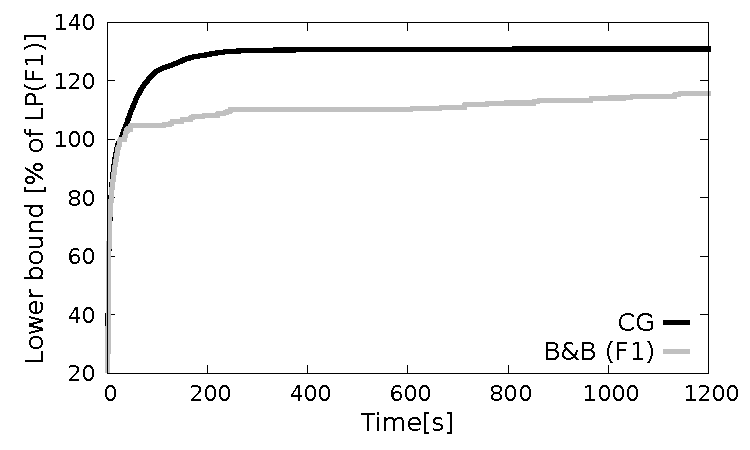
\includegraphics[width=\textwidth]{lower-bound-24-12}
        \caption{$|V|=24, |D|=12$}
        \label{fig:cggr24-12}
    \end{subfigure}
    \hfill %add desired spacing between images, e. g. ~, \quad, \qquad, \hfill etc. 
      %(or a blank line to force the subfigure onto a new line)
    \begin{subfigure}[b]{0.49\textwidth}
        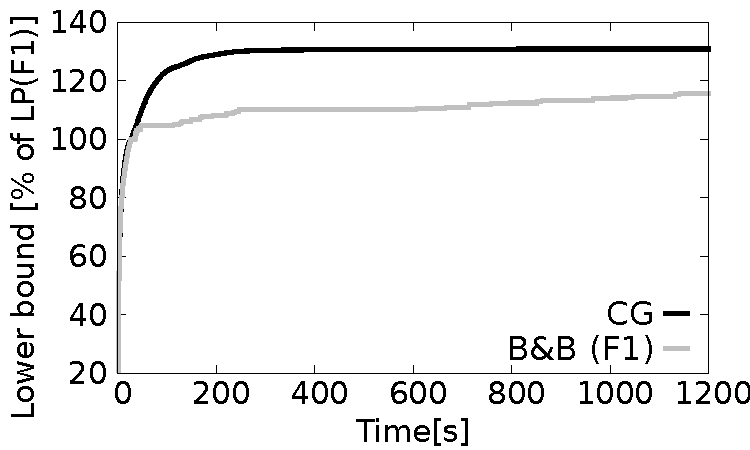
\includegraphics[width=\textwidth]{lower-bound-26-13}
        \caption{$|V|=26, |D|=13$}
        \label{fig:cggr26-13}
    \end{subfigure}
  
    \begin{subfigure}[b]{0.49\textwidth}
        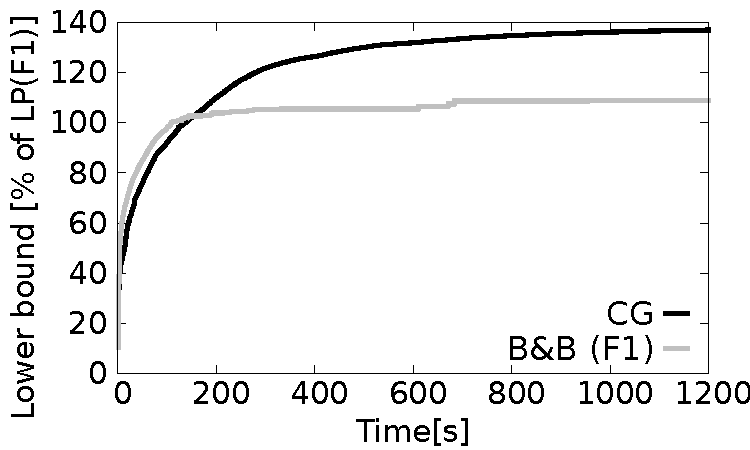
\includegraphics[width=\textwidth]{lower-bound-28-14}
        \caption{$|V|=28, |D|=14$}
        \label{fig:cggr28-14}
    \end{subfigure}
    \hfill %add desired spacing between images, e. g. ~, \quad, \qquad, \hfill etc. 
      %(or a blank line to force the subfigure onto a new line)
    \begin{subfigure}[b]{0.49\textwidth}
        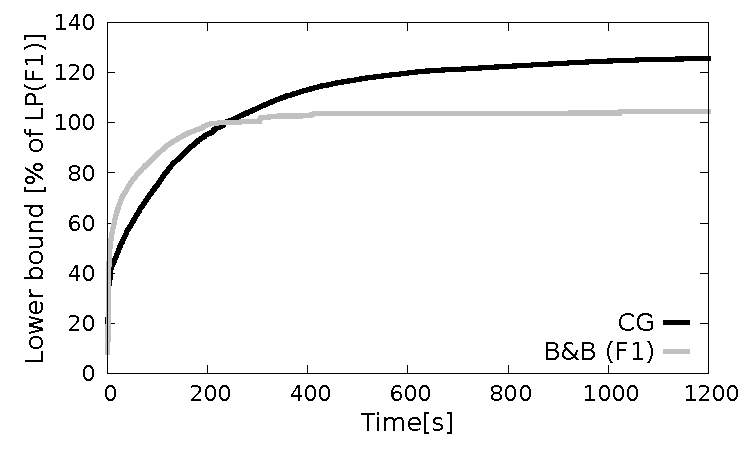
\includegraphics[width=\textwidth]{lower-bound-30-15}
        \caption{$|V|=30, |D|=15$}
        \label{fig:cggr30-15}
    \end{subfigure}

    \begin{subfigure}[b]{0.49\textwidth}
        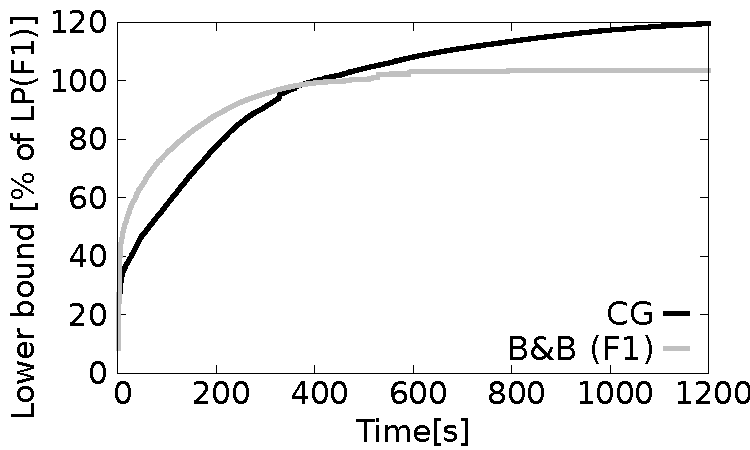
\includegraphics[width=\textwidth]{lower-bound-32-16}
        \caption{$|V|=32, |D|=16$}
        \label{fig:cggr32-16}
    \end{subfigure}
    \hfill %add desired spacing between images, e. g. ~, \quad, \qquad, \hfill etc. 
      %(or a blank line to force the subfigure onto a new line)
    \begin{subfigure}[b]{0.49\textwidth}
        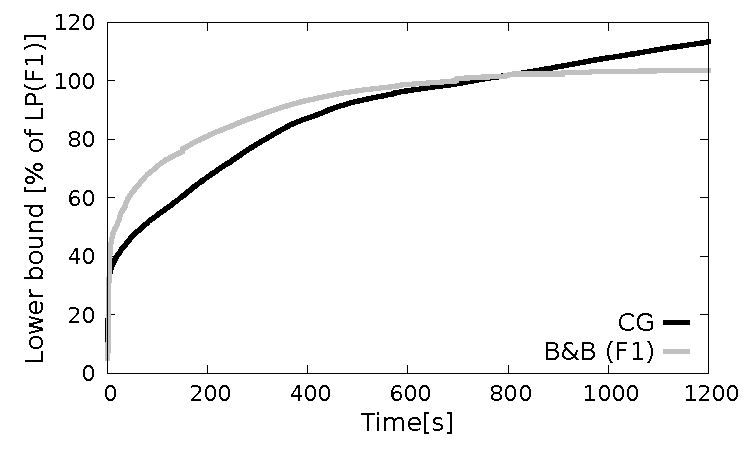
\includegraphics[width=\textwidth]{lower-bound-34-17}
        \caption{$|V|=34, |D|=17$}
        \label{fig:cggr34-17}
    \end{subfigure}
  \caption{Comparison of lower bounds obtained by CG and B\&B on model $\mathcal{F}_1$.
	\textcolor{blue}{Each figure depicts a progress of lower bounds for instances with varying number of destination and non-destination nodes.
	The lower bounds are obtained by solving CG scheme applied on model $\mathcal{F}_1$ (black curves), and produced during the course of classic B\&B algorithm (grey curves)
	The tightness of the bounds increases with time, and it can be observed from the graphs that the CG bound becomes tighter at some point.
	We express the quality of lower bounds with respect to the value of simple continuous relaxation, as indicated by the vertical axes.
	It can also be noted that the lower bound obtained from B\&B grows sharply during the computation of the simplex method in the root of the B\&B tree, 
	which is happening until the curve reaches 100\%.
	After that point the bound grows rather slowly.
	CG on the other hand produces bound that grows faster even after the value of first relaxation in the root is reached.
%	The values can be retrieved from the output of CPLEX during the course of simplex and B\&B algorithm.
	}}
  \label{fig:cggr}
\end{figure} 

Reflecting the progress of the dual simplex method applied to $\text{LP}(\mathcal{X}_2)$ and $\text{LP}(\mathcal{F}_1)$, respectively,
both CG and B\&B increase the lower bound sharply at the beginning. 
While solution of $\text{LP}(\mathcal{F}_1)$ is still in progress, the growth of the lower bound is faster than what is observed for CG (solution of $\text{LP}(\mathcal{F}_1)$). 
This is particularly apparent for instances of size 28 and larger (Fig. \ref{fig:cggr28-14} - \ref{fig:cggr34-17}). %and can be explained as a consequence of Prop. \ref{prop:f1strx1}.
Once $\text{LP}(\mathcal{F}_1)$ is solved, the increase slows down substantially, and remains modest until the time limit is reached. 
An analogous, but more moderate, gradual slow-down is also observed for CG.
In each instance set, the two curves intersect at some point in time.
From this moment on, CG provides a tighter lower bound.
Experiments reported in Fig.\ \ref{fig:cggr} thus indicate that CG is the more suitable method for obtaining tight lower bounds within a given time.
